\documentclass{article}
\usepackage{graphicx}
\usepackage{hyperref}
\usepackage{geometry}
\geometry{a4paper, margin=1in}

\title{Full Progress Report: FRB Host Galaxy Analysis}
\author{GitHub Copilot}
\date{\today}

\begin{document}

\maketitle

\section{Photutils Inclination Analysis}
Comparison between \texttt{photutils}, GALFIT, and SDSS inclinations.

\begin{figure}[h!]
    \centering
    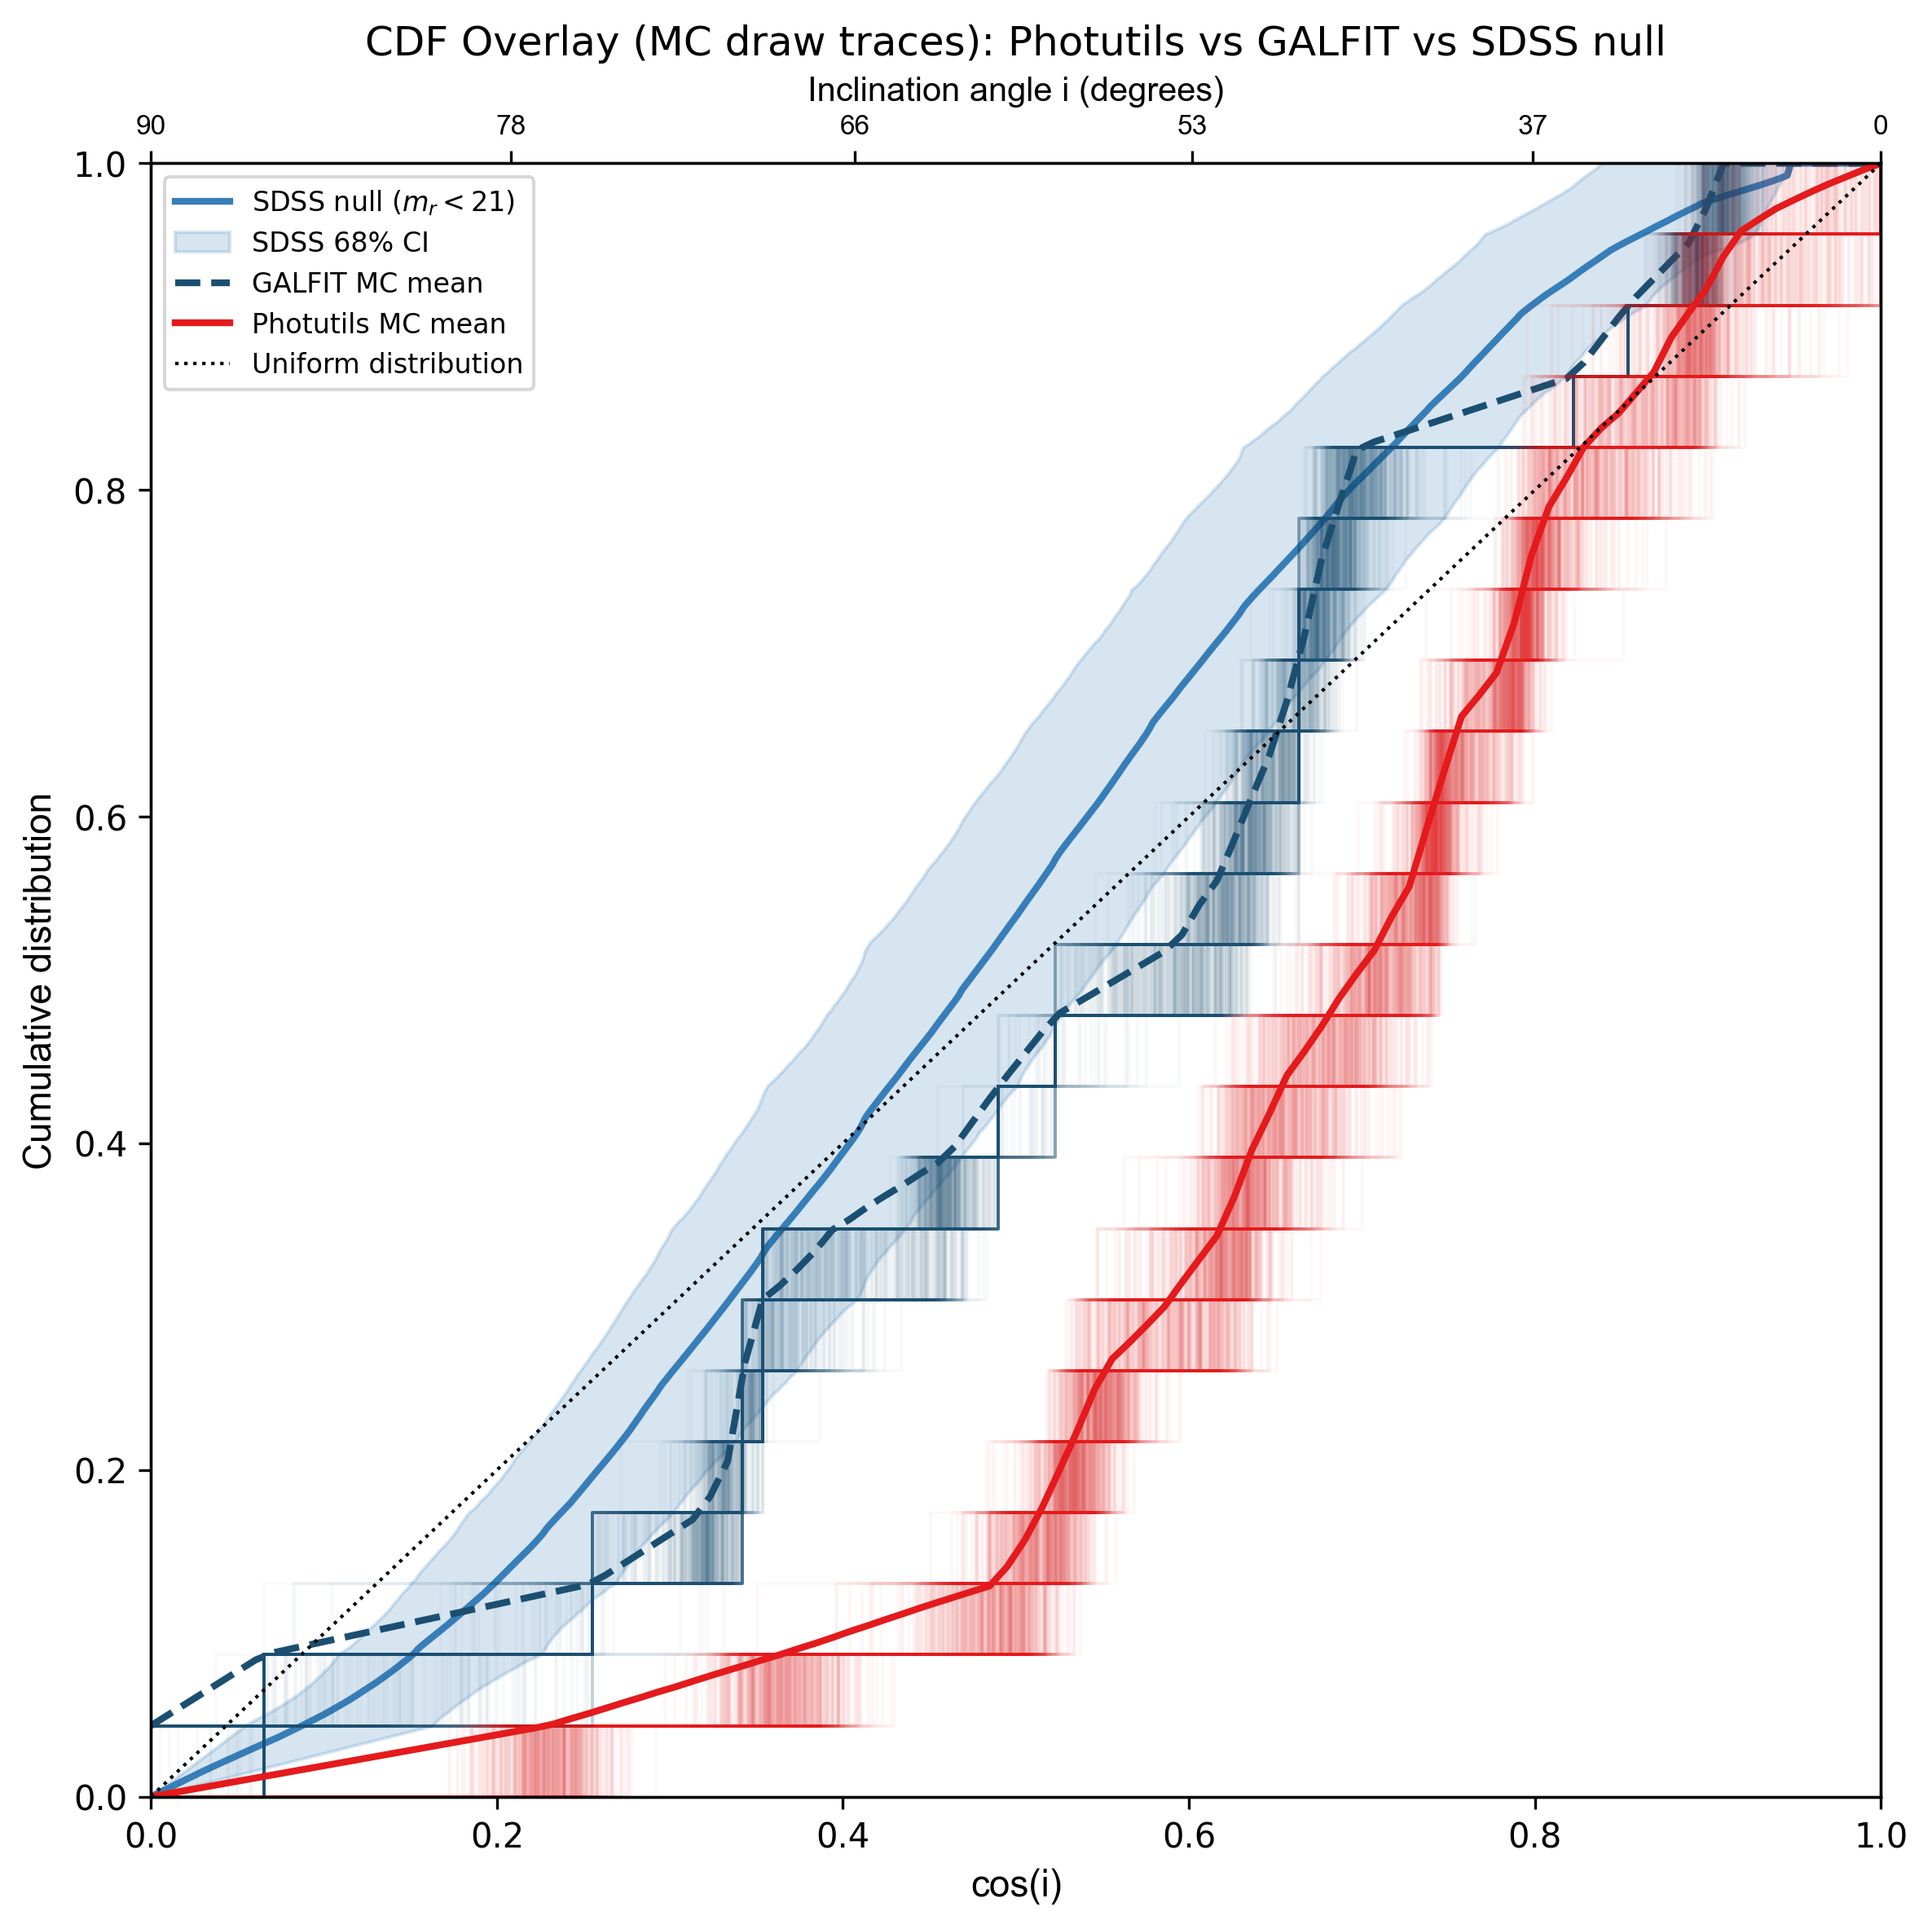
\includegraphics[width=0.8\textwidth]{images/photutils_vs_galfit_vs_sdss_nopsf_spaghetti.png}
    \caption{GALFIT and Photutils inclination comparisons against SDSS, including Monte Carlo uncertainty tracks.}
    \label{fig:mc_comparison}
\end{figure}

\begin{figure}[h!]
    \centering
    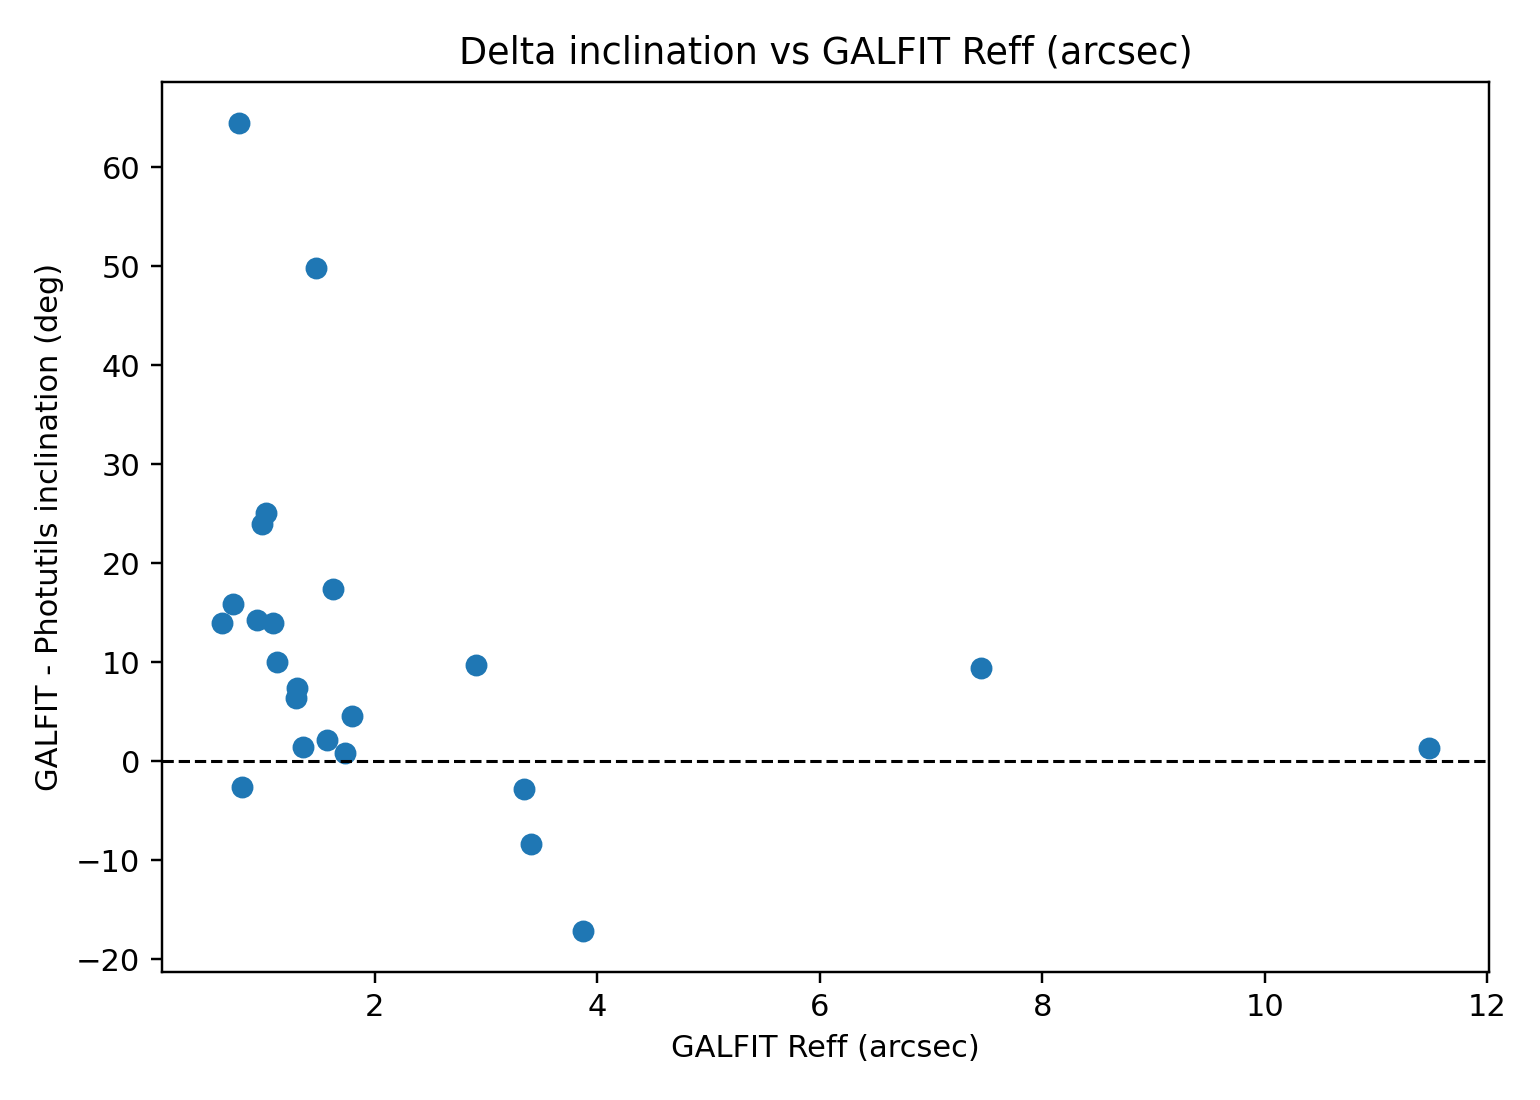
\includegraphics[width=0.8\textwidth]{images/delta_inc_galfit_minus_photutils_vs_galfit_reff_arcsec.png}
    \caption{Difference in inclination (GALFIT - Photutils) vs. GALFIT effective radius in arcseconds.}
    \label{fig:delta_inc_reff}
\end{figure}

\begin{figure}[h!]
    \centering
    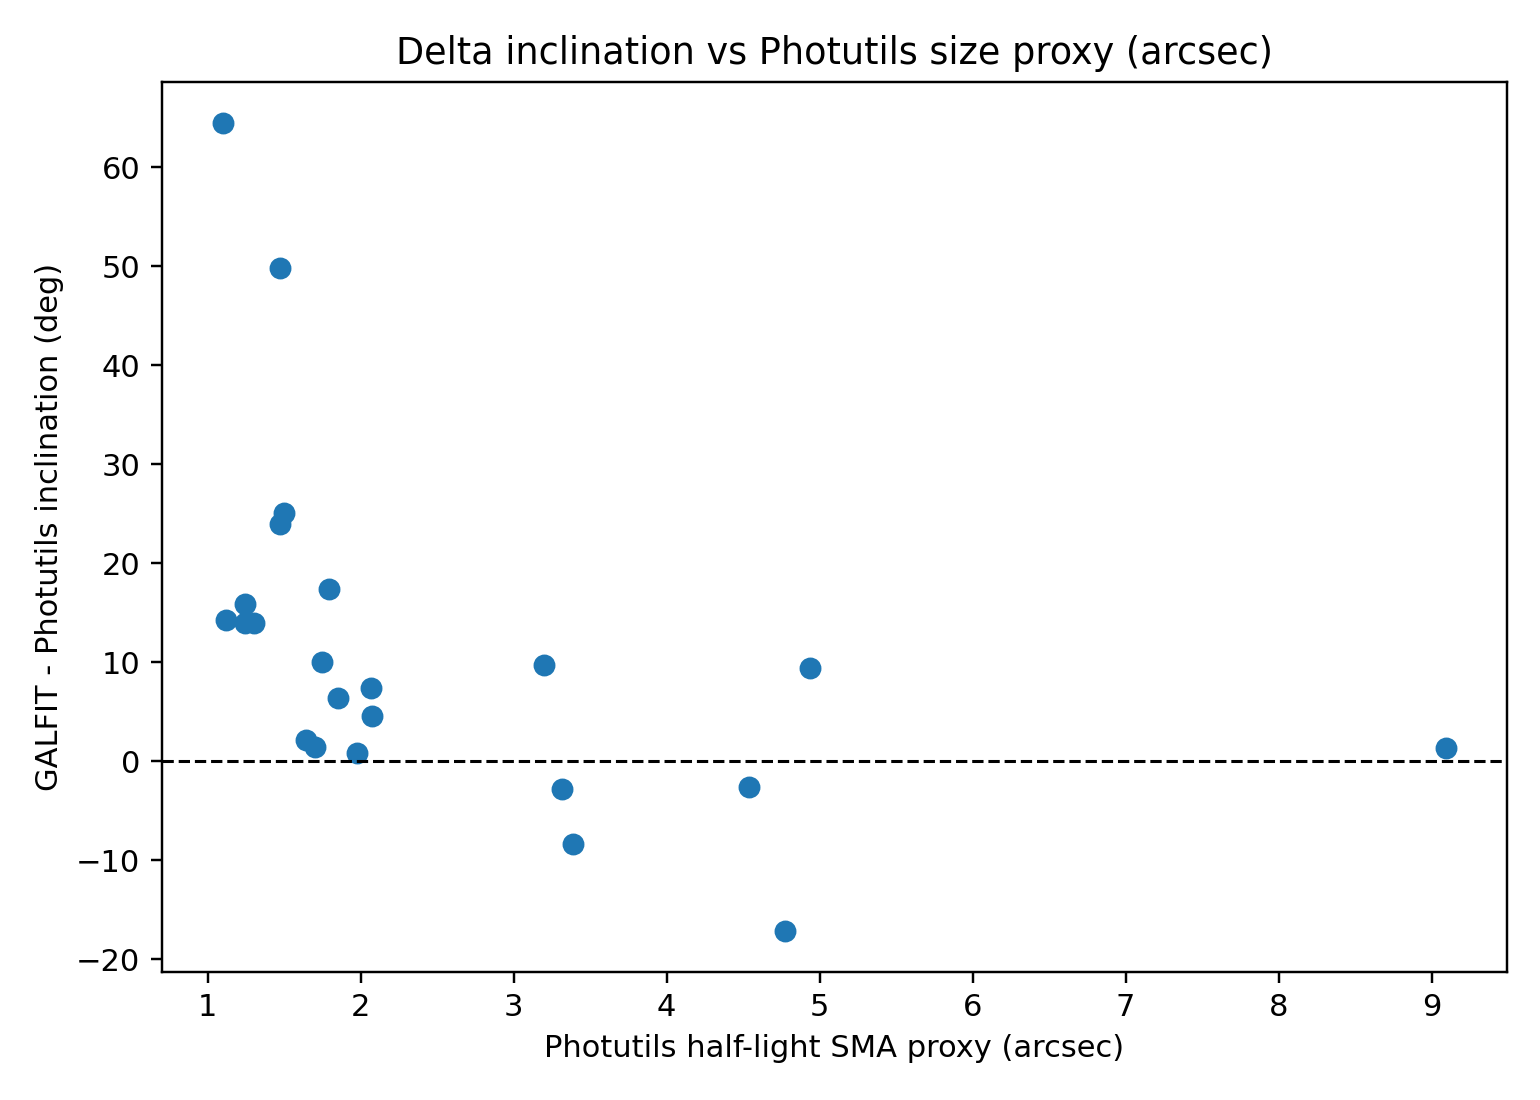
\includegraphics[width=0.8\textwidth]{images/delta_inc_galfit_minus_photutils_vs_photutils_sma_proxy_arcsec.png}
    \caption{Difference in inclination (GALFIT - Photutils) vs. Photutils semi-major axis proxy in arcseconds.}
    \label{fig:delta_inc_sma}
\end{figure}

\clearpage

\section{Legacy Survey vs. GALFIT Comparison}
\noindent Even as \(n\) changes massively, \(R_{\mathrm{eff}}\) remains nearly the same in Legacy Survey fits; with model and residual images looking so similar, the fitting behavior is confusing.

\input{legacy_vs_galfit_selected_fields_all_rows_table.tex}

\noindent Legacy tends to fit very low-SNR regions, which can break up galaxies (as seen in the largest-deviation cases); GALFIT still provides the better fit overall.

\begin{figure}[p]
    \centering
    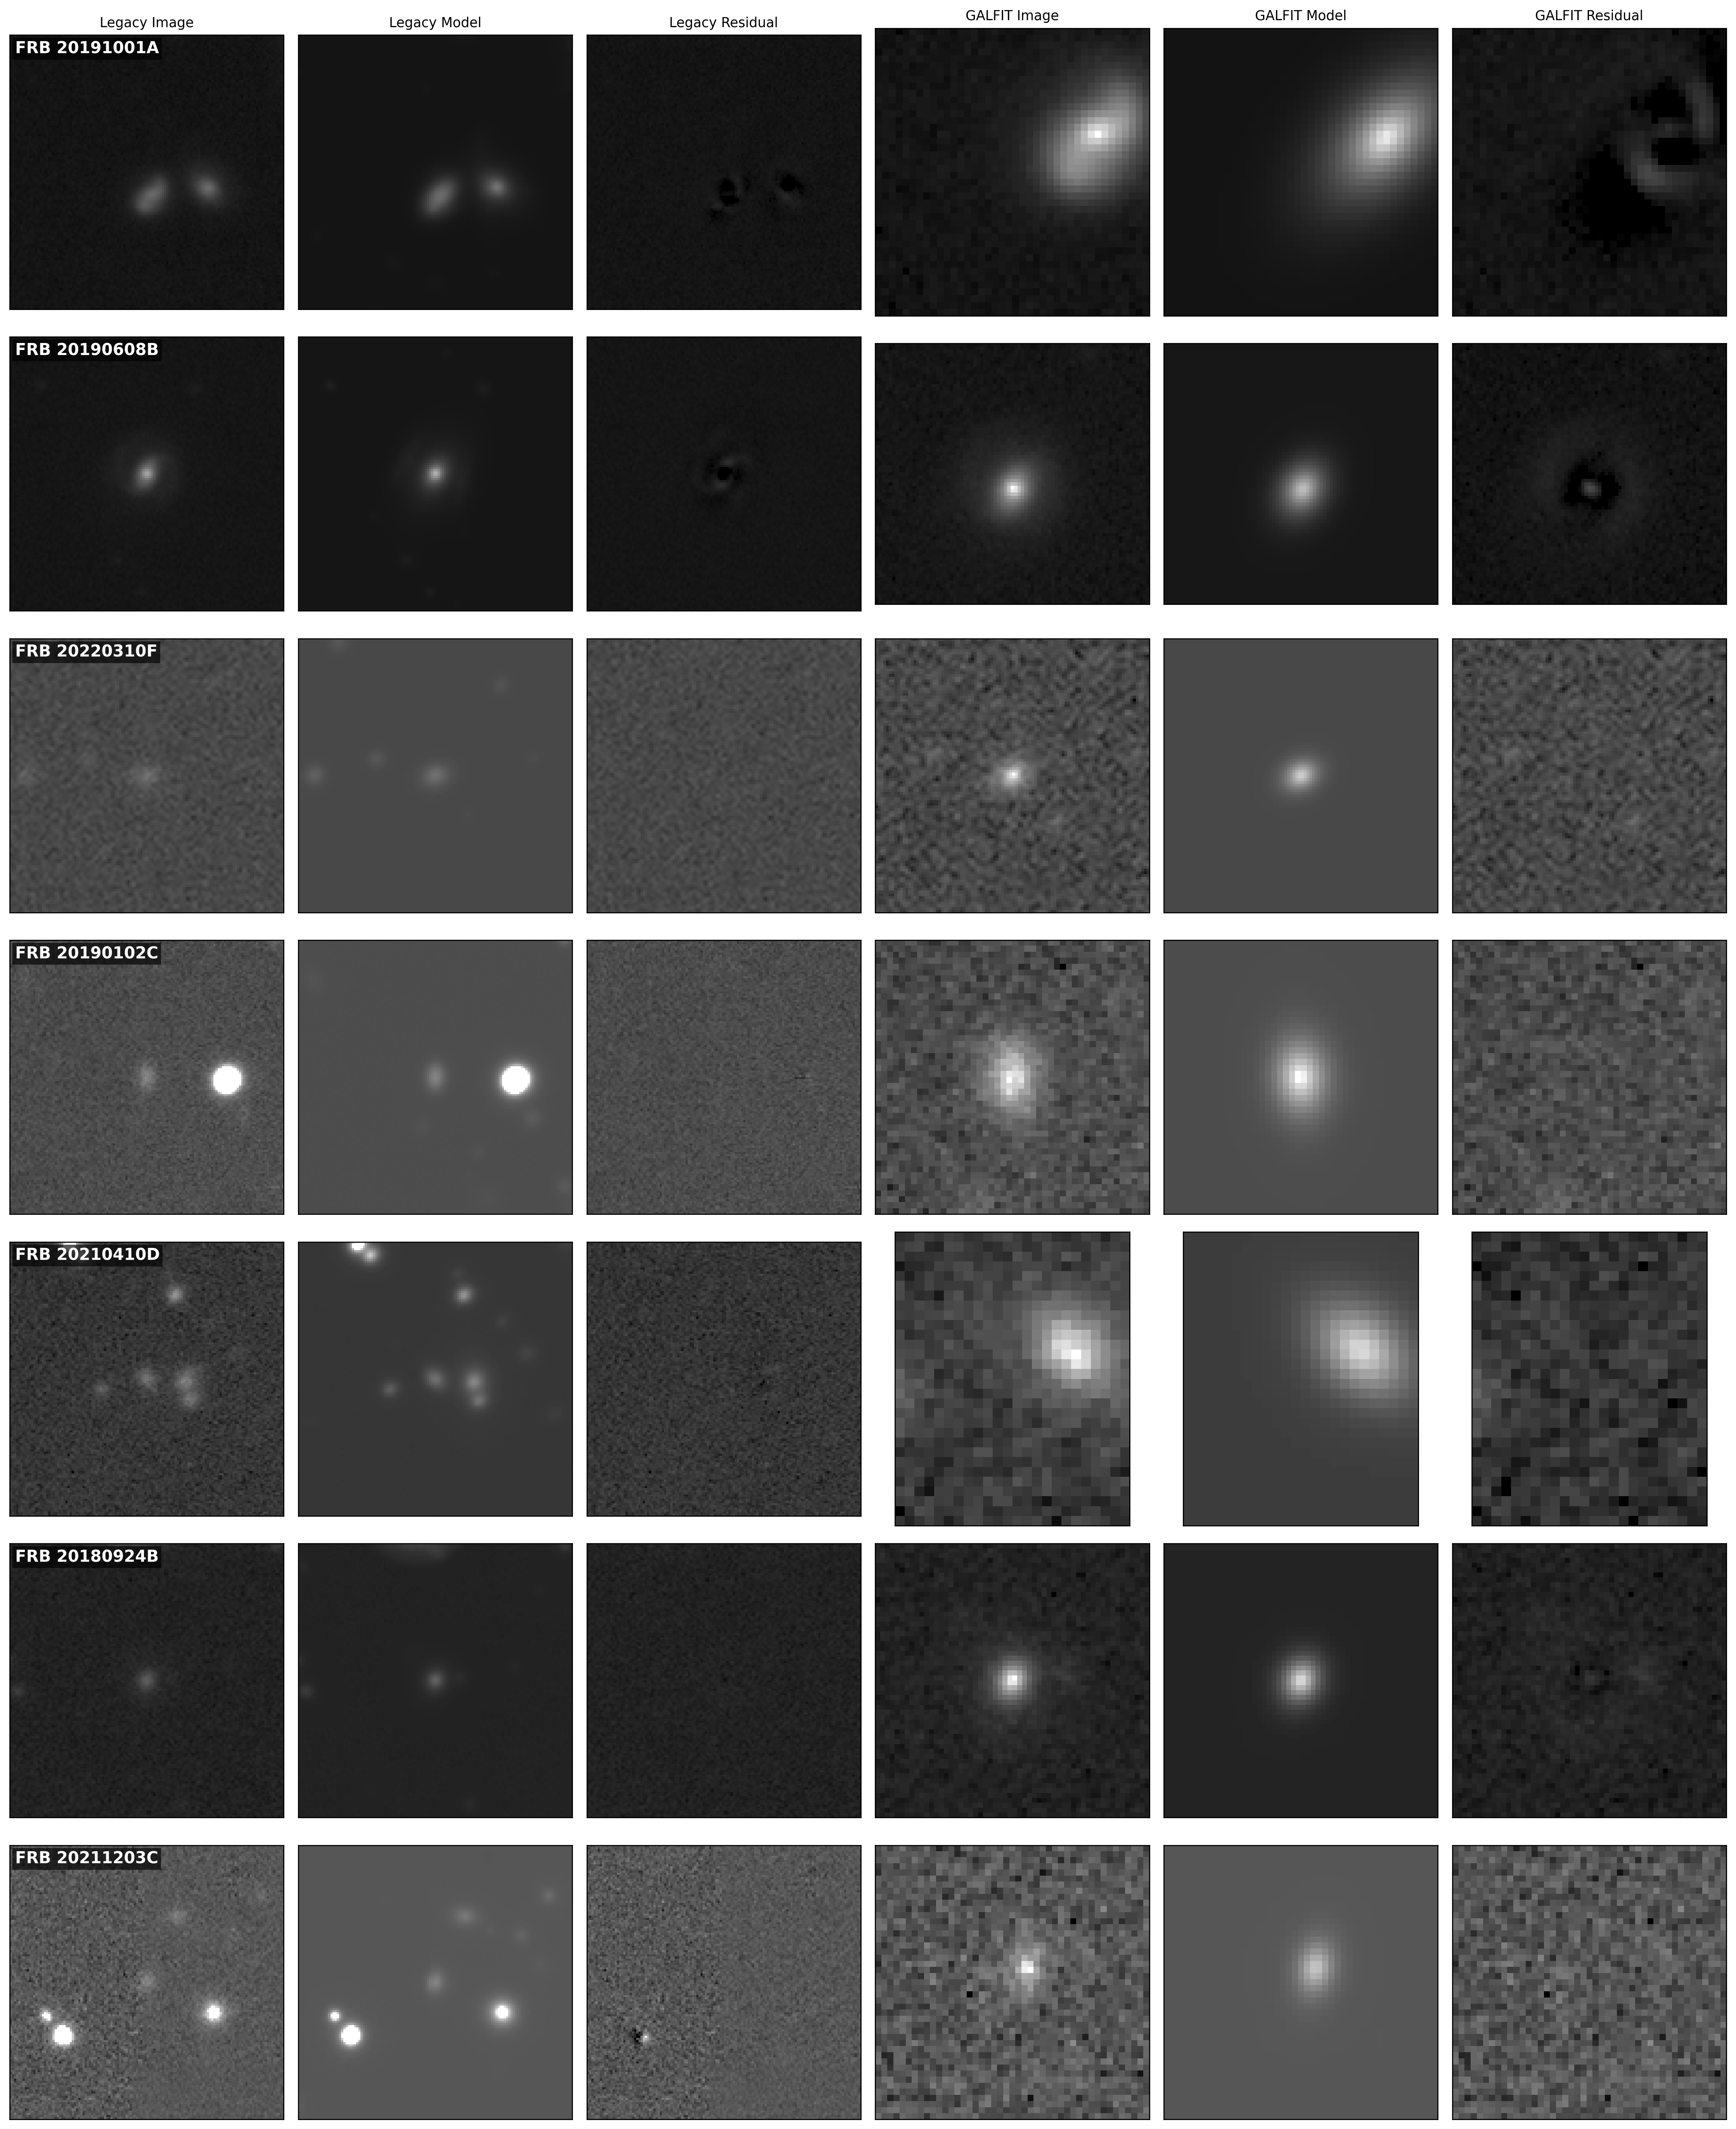
\includegraphics[width=\textwidth,height=0.86\textheight,keepaspectratio]{images/panel_top_delta_i_no_rex_13_part1.png}
    \caption{Top 7 non-REX Legacy-vs-GALFIT IMR diagnostics, with FRB names shown on each row.}
    \label{fig:imr_panel_full_nonrex_part1}
\end{figure}

\begin{figure}[p]
    \centering
    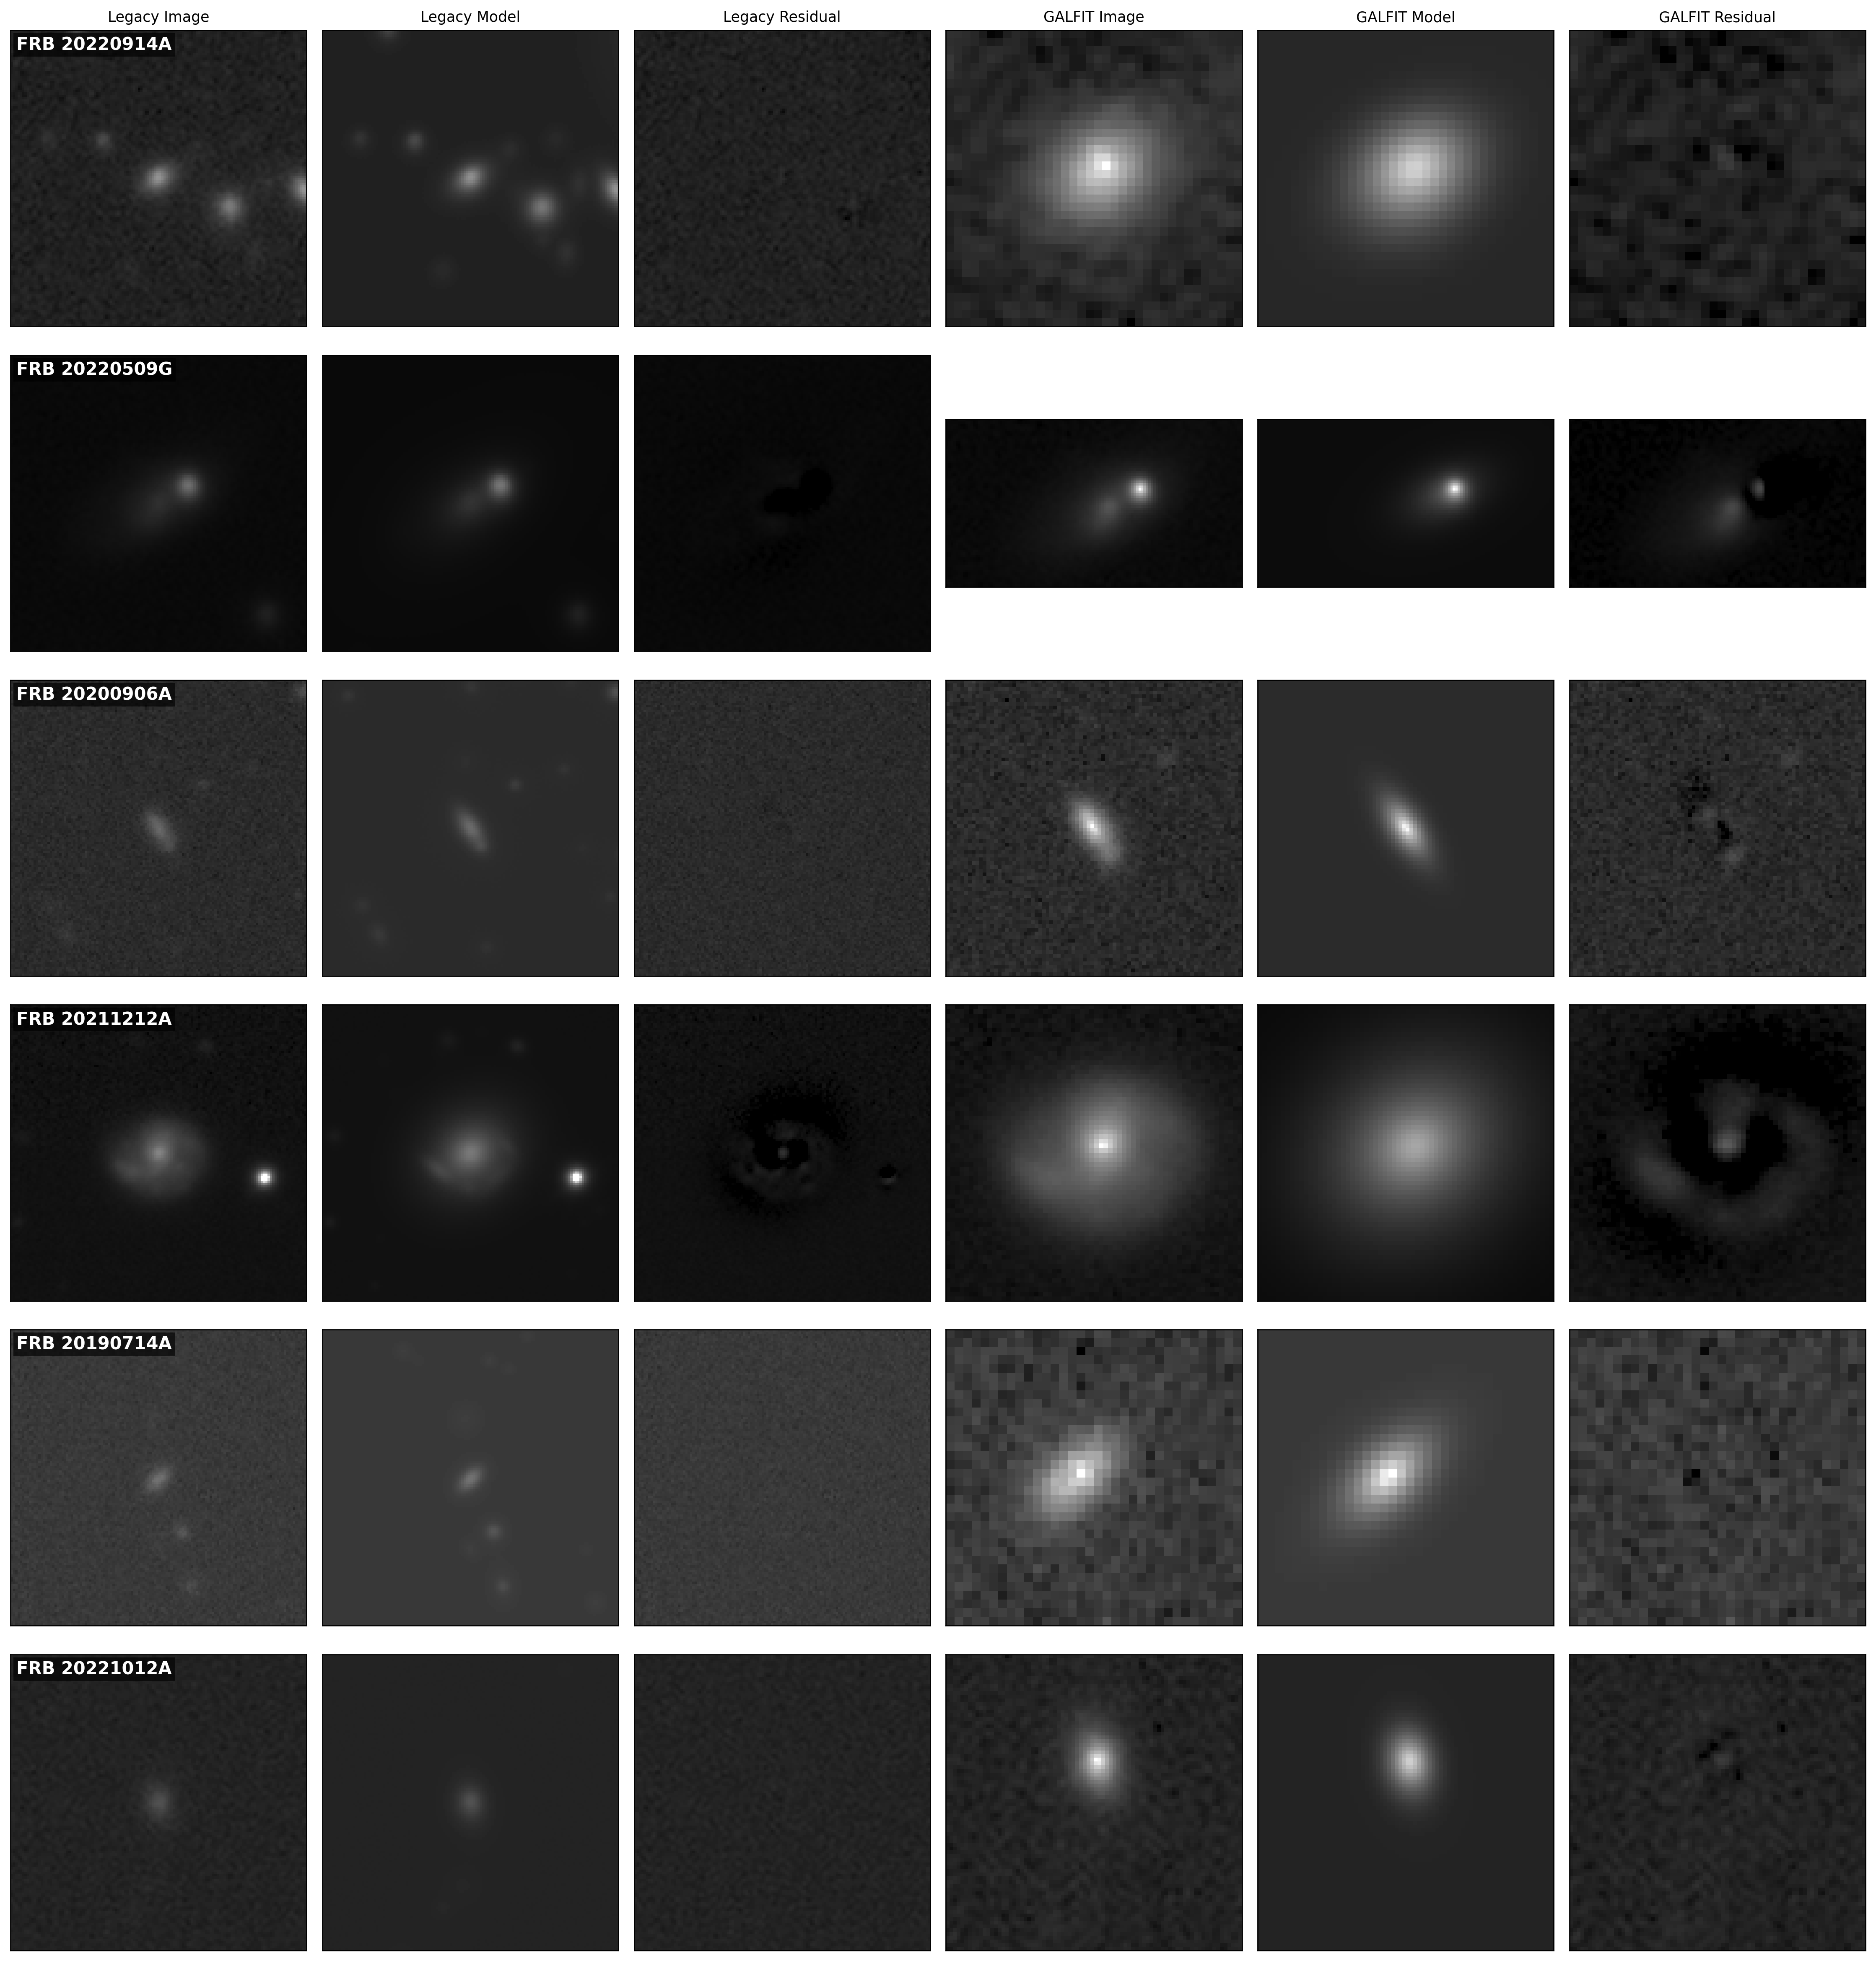
\includegraphics[width=\textwidth,height=0.86\textheight,keepaspectratio]{images/panel_top_delta_i_no_rex_13_part2.png}
    \caption{Remaining 6 non-REX Legacy-vs-GALFIT IMR diagnostics, with FRB names shown on each row.}
    \label{fig:imr_panel_full_nonrex_part2}
\end{figure}

\clearpage



\end{document}
